\section{Fallbeschleunigung und Trägheitsmoment eines Fallrades} 

	Das Fallrad verhält sich wie das Jo-Jo Spielzeug. Lässt man das aufgewickelte Fallrad fallen, bei festgehaltener Schnur, so fällt es langsamer und und wickelt sich nach Abwickeln der Schnur von selbst wieder auf. In diesem Versuch werden die Fallbeschleunigung und das Trägheitsmoment eines Fallrades bestimmt und überprüft, ob die gemessenen und bestimmten Werte mit den aus der Theorie berechneten Werten übereinstimmen. Dazu wird angenommen, dass die aus der Theorie bekannten Formeln den Sachverhalt korrekt beschreiben. Das Ergebnis dieses Versuches stimmt mit diesen überein. 
	
	\subsection{Methoden}
		
		\subsubsection{Aufbau}
		
			\begin{figure}[ht]
				\centering
				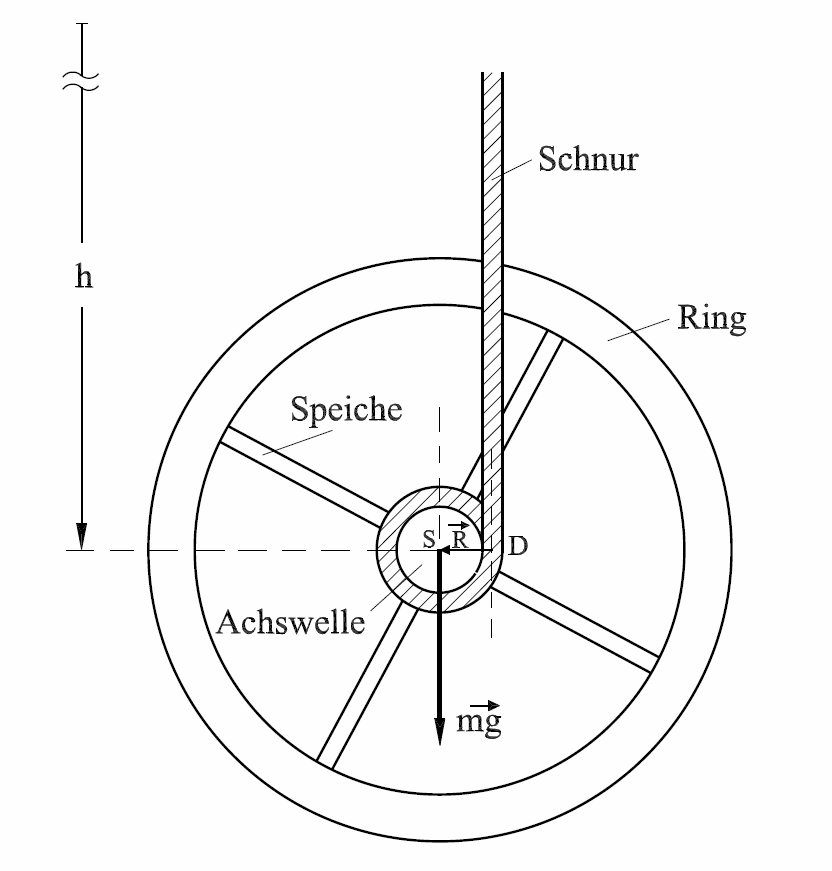
\includegraphics[width=0.7\textwidth]{fallrad_skizze.png}
				\caption{Die Versuchsskizze zeigt den Aufbau des Fallrades aus der Seitenansicht.}
				\label{fig:FallradSkizze}	
			\end{figure}
			Es wird der in Abb. \ref{fig:FallradSkizze} dargestellte Aufbau betrachtet. 
			Das Fallrad besteht aus einem Ring, in dessen Mittelpunkt sich die Achse befindet, um welche die Bewegung durchgeführt wird. Mit Hilfe von vier Speichen ist der Ring mit der Achse verbunden. Zur Vereinfachung wird angenommen, dass es sich hierbei um zwei senkrecht zueinander liegende Zylinder handelt, die in ihren Mittelpunkten mit der Achse verbunden sind. 
			Die Achse liegt mittig in dem Ring, sodass die Schnur auf beiden Seiten mit dem gleichen Abstand von dem Ring angebracht werden kann (vgl. \ref{fig:FallradFrontal}). 
			\begin{figure}[ht]
				\centering
				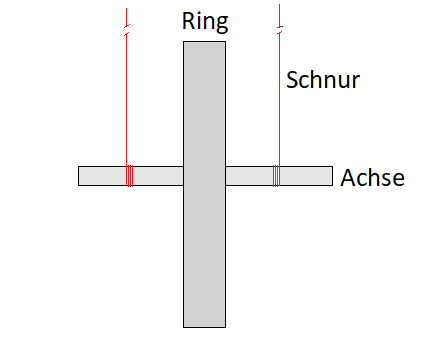
\includegraphics[width=0.6\textwidth]{fallrad_frontal.png}
				\caption{Die Versuchsskizze zeigt die Frontalansicht des Aufbaus. Hierbei ist die Achse zu erkennen, auf der sich der Faden auf-/abrollt.}
				\label{fig:FallradFrontal}	
			\end{figure}
			In der Ruhelage liegen keine Wicklungen der Schnur auf der Achse vor. Die Größe $h$ gibt die Höhe des Fallrades, als Abstand von der Ruhelage, an. 
		
		\subsubsection{Durchführung}
			
			Mit einer Stoppuhr wird die Zeit gemessen, die das Fallrad benötigt bis keine Wicklung des Fadens auf der Achse vorliegt. Dies wird für verschiedene Starthöhen durchgeführt um die Fallbeschleunigung $g^{*}$ zu bestimmen. Dafür ist es wichtig darauf zu achten, dass die Schnur sich bei dem Aufwickeln nicht auf sich selber, sondern nur auf der Achse wickelt, damit sich der Abrollradius nicht verändert.
			Die Höhe wird von einem Maß abgelesen, wobei das Fallrad in Ruhelage (bzw. wenn keine Wicklung des Fadens auf der Achse vorliegt) bei genau \SI{0}{\cm} an dem Maß liegt. 
			
			Zur Bestimmung des Trägheitsmoments werden die Maße des Fallrads mit Hilfe einer Schiebelehre gemessen und die Masse gewägt.			
			
		\subsubsection{Unsicherheiten}
			
			Im Allgemeinen dient zur Berechnung der Unsicherheiten für die gemessenen und ermittelten Werte folgende Formel: 
			\begin{equation*}
				u(s) = \pm \sqrt{\sum_{k=0}^{N}\left( \frac{\partial f}{\partial x_i}u(x_i)\right) ^2}. \label{eq:kombUnsicherheit}
			\end{equation*}
			Für die Messunsicherheit der Stoppuhr wird aufgrund der Digitalanzeige eine Rechtecksverteilung verwendet und diese dann mit der Unsicherheit für die Reaktionszeit\footnote{hierzu werden \SI{0.1}{\s} dreiecksverteilt verwendet} kombiniert. Die Schiebelehre besitzt eine Messgenauigkeit von \SI{0,02}{\mm}, da sich so genau jedoch nicht ablesen lässt, wird eine Dreicksverteilung über \SI{0,04}{\mm} verwendet. Für das Maß wird ebenfalls eine Dreiecksverteilung gewählt, hierbei über \SI{1}{\mm}.
			Die Berechnung der Unsicherheiten liegt im Anhang (\ref{Anhang})  vor, da diese für einige Größen umfangreicher ist.
			
	\subsection{Messung}
	
		\subsubsection{Messwerte}
			
			Die in Tab. \ref{tab:Messwerte} dargestellten Werte sind die (gemittelten) Messwerte, welche aufgenommen wurden. Dabei ist die Berechnung der verwendeten kombinierten Unsicherheiten, für z. B. die gemittelten Werte, dem Anhang zu entnehmen.
			\begin{table}[ht]
				\caption{In dieser Tabelle sind die gemessenen Werte verzeichnet. Die Größen welche mehrmals gemessen wurden, sind hier gemittelt.}
				\centering
				\label{tab:Messwerte}
				\begin{tabular}{l c}
					{Maße des Fallrads} &
					\begin{tabular}{l l}
						\begin{tabular}{l|l}
							{Größe} & {Wert}	\\
							\hline
							{Dicke $H$ des Rings} & {\SI{11,68+-0,03}{\mm}} \\
							{Außenradius $R_a$ des Rings} & {\SI{90,08+-0,01}{\mm}} \\
							{Innenradius $R_i$  des Rings} & {\SI{77,59+-0,01}{\mm}} \\
							{Speichenradius $R_S$} & {\SI{3,490+-0,006}{\mm}} \\
							{Achsenradius $R_A$} & {\SI{4,090+-0,006}{\mm}} \\
							{Achsenlänge $L_A$} & {\SI{200,3+-0,002}{\mm}} \\
							{Masse $m$} & {\SI{768,16+-0,01}{\g}} \\
							{Fadendicke $d$} & {\SI{1,027+-0,028}{\mm}} \\
						\end{tabular}	
					\end{tabular}
					\\ & \\
					{Fallhöhe und Fallzeit} &
					\begin{tabular}{l|l}
						{Fallhöhe $h$} & {Fallzeit $t$}	\\
						\hline
						{\SI{200+-0,29}{\mm}} & {\SI{3,402+-0,046}{\s}} \\
						{\SI{350+-0,29}{\mm}} & {\SI{4,488+-0,046}{\s}} \\
						{\SI{500+-0,29}{\mm}} & {\SI{5,286+-0,046}{\s}} \\
						{\SI{650+-0,29}{\mm}} & {\SI{6,122+-0,046}{\s}} \\
						{\SI{800+-0,29}{\mm}} & {\SI{6,782+-0,046}{\s}} \\
					\end{tabular}
				\end{tabular}					
			\end{table}
			
		\subsubsection{Messergebnisse}	
			
			\begin{figure}[ht]
				\centering
				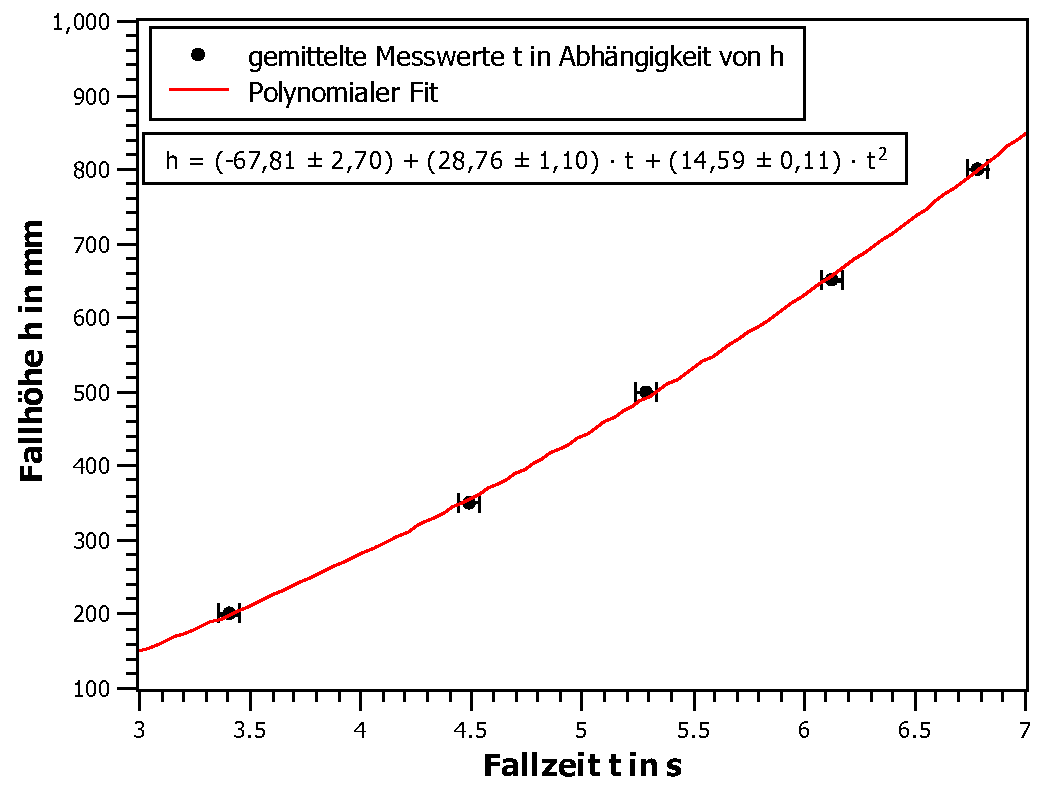
\includegraphics[width=\textwidth]{h-gegen-t.pdf}
				\caption{Graphische Darstellung der Fallhöhe $h$ in Abhängigkeit der Fallzeit $t$.}
				\label{fig:hgegent}	
			\end{figure}
			In dem Ersten der drei folgenden Diagrammen (Abb. \ref{fig:hgegent}) ist die Fallhöhe $h$ gegen die Fallzeit $t$ aufgetragen.
			Aufgrund des leicht gekrümmten Verlaufs und der Formel zur Berechnung der Fallhöhe
			\begin{equation}
				h(t) = \frac{1}{2}g \frac{mR^2}{J_S + mR^2} t^2 = \frac{1}{2}g^{*}t^2 \label{eq:Fallbeschleunigung}
			\end{equation}
			wurde ein polynomialer Fit\footnote{Dieser Fit und seine Unsicherheit, wie auch die der nächsten beiden, wurde von dem Programm SciDavis berechnet, dazu wurden die Unsicherheiten (welche im Anhang zu finden sind) und die Methode der kleinsten Quadrate herangezogen} für das Diagramm gewählt.
			Der Fit besitzt folgende Form: 
			\begin{equation*}
				h(t) = [(-67,81\pm 2,70)+(28,76\pm 1,10)t\cdot\si{s^{-1}}+(14,59\pm 0,11)t^2\cdot\si{s^{-2}}]\si{\mm}.
			\end{equation*} 
			\begin{figure}[ht]
				\centering
				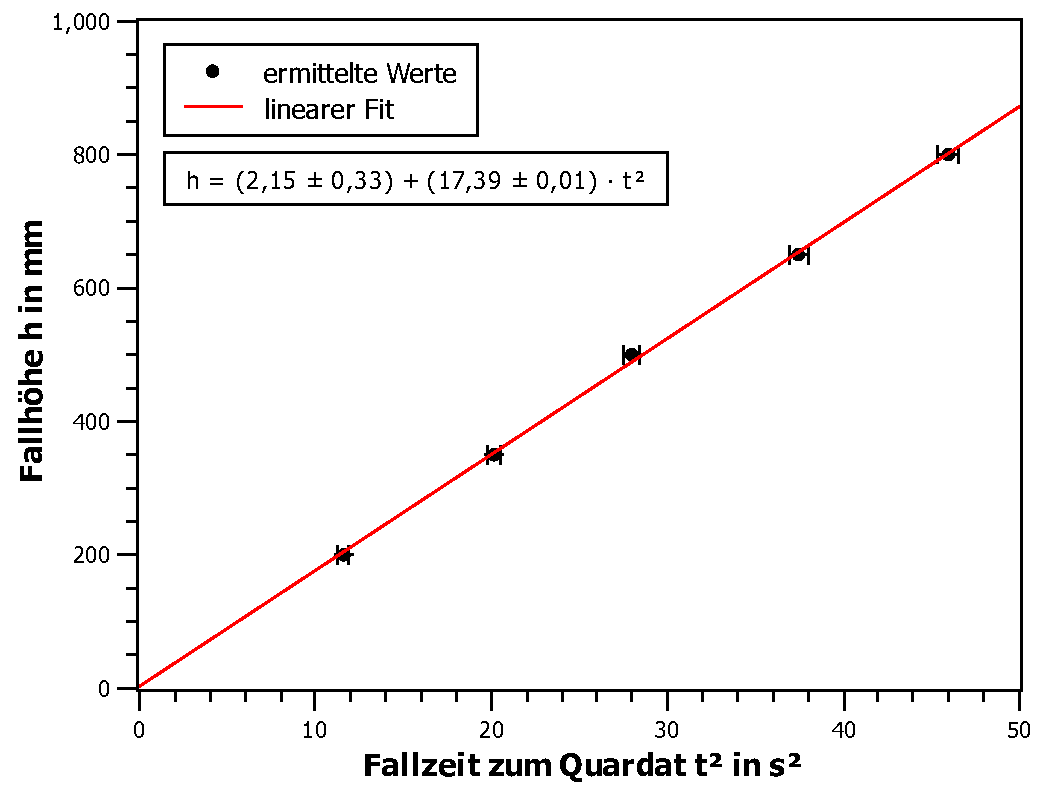
\includegraphics[width=\textwidth]{h-gegen-t2.pdf}
				\caption{Graphische Darstellung der Fallhöhe $h$ in Abhängigkeit der quadrierten Fallzeit $t^2$.}
				\label{fig:hgegent2}	
			\end{figure}	
			Da im zweiten Diagramm die Fallhöhe $h$ gegen die quadrierte Fallzeit $t^2$ aufgetragen ist, sollte sich hierbei nach obiger Gleichung ein linearer Zusammenhang zeigen. Aus diesem Grund wurde für dieses Diagramm ein linearer Fit gewählt. Hierbei sollte die Steigung nach Gl. \ref{eq:Fallbeschleunigung} gerade gleich der halben Fallbeschleunigung $g^{*}$ entsprechen. Folgende Formel beschreibt den Fit:
			\begin{equation*}
				h(t) = [(2,15 \pm 0,33)+(17,39 \pm 0,01)t^2\cdot\si{s^{-2}}]\si{\mm}.
			\end{equation*} 
			\begin{figure}[ht]
				\centering
				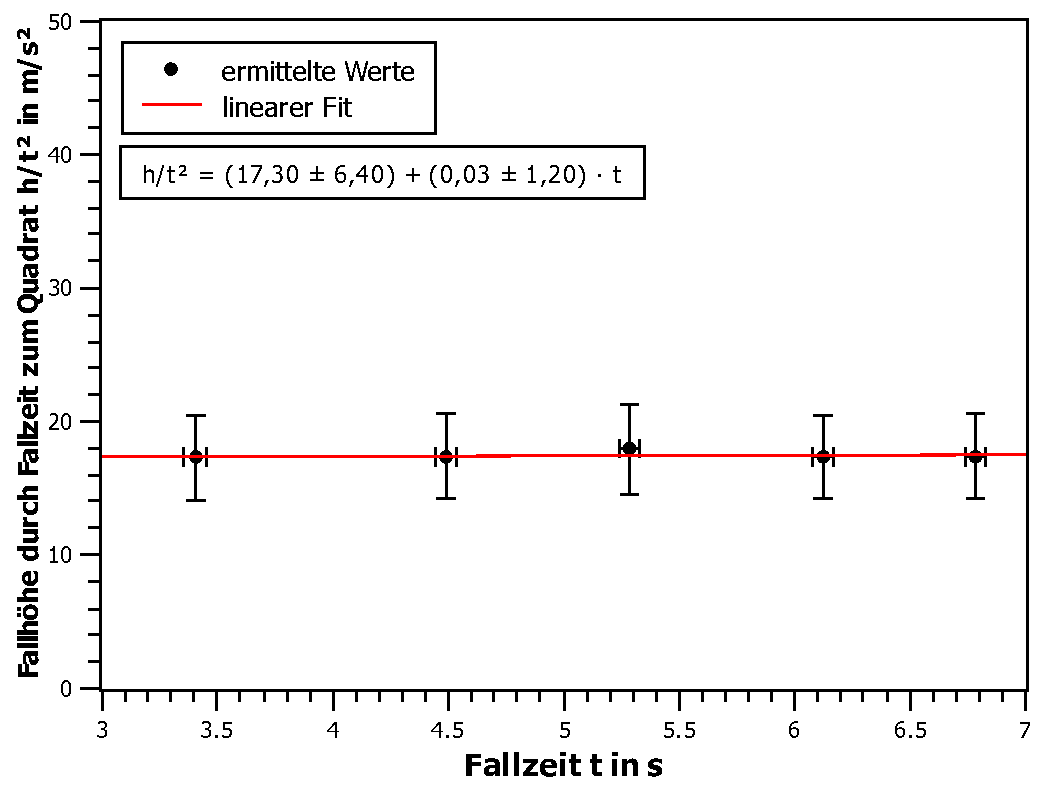
\includegraphics[width=\textwidth]{ht2-gegen-t.pdf}
				\caption{Graphische Darstellung der Fallhöhe geteilt durch die quadrierte Fallzeit $\frac{h}{t^2}$ in Abhängigkeit der Fallzeit $t$.}
				\label{fig:ht2gegent}	
			\end{figure}
			Da diese Steigung nicht von der Zeit abhängt, ist wie in dem letzten Diagramm näherungsweise zu sehen $\frac{h}{t^2}$ konstant. Auch hier wurde aufgrund dieses Verhaltens ein linearer Fit gewählt. Da die ermittelten Punkte auf einer Horizontalen liegen zu scheinen ist die Steigung demnach $\approx 0$. Aufgrund der Unsicherheit, welche merklich von null entfernt ist, wird dies jedoch nicht ganz gestützt. Der Fit sieht wie folgt aus:
			\begin{equation*}
				\frac{h}{t^2} = [(17,30 \pm 6,40) + (0,03 \pm 1,20)t\cdot\si{s^{-1}}]\si{\mm}.
			\end{equation*} 
			Wählt man die Steigung gleich null und multipliziert man das Ergebnis mit zwei, so ergibt sich für $g^{*} = \SI{34,6+-12,8}{\m\per\s^2}$. 
					
			Zur Bestimmung des Trägheitsmoments $J_S$ des Fallrads werden die Trägheitsmomente der Bestandteile addiert. Diese lassen sich durch Zylinderträgheitsmomente bestimmen. Für den Ring wird die Formel für einen Hohlzylinder verwendet, welcher parallel zur Drehachse liegt:
			\begin{align}
					J_{parallel} = \frac{1}{2}\pi H\rho(R_a^4-R_i^4). \label{eq:Trägpar}
			\end{align}
			Ebenso lässt sich das Trägheitsmoment der Achse bestimmen, da es sich hierbei jedoch um einen Vollzylinder handelt wird der Innenradius in der Formel gleich null gesetzt.
			Für die vier Speichen wird vereinfacht, so dass nur zwei Zylinder senkrecht zur Drehachse betrachtet werden.
			Dieses bestimmt sich wie folgt: 
			\begin{align}
				J_{senkrecht} = \pi H\rho\left[\frac{1}{12}H^2R^2+\frac{1}{4}R^4\right]. \label{eq:Trägsenk}
			\end{align} 
			Zur Bestimmung der Dichte muss das Volumen bestimmt werden und die gemessene Masse dadurch geteilt werden. Das Volumen setzt sich wie auch das Trägheitsmomenten aus den Einzelteilen zusammen:
			\begin{equation}
				V = V_{Ring} + 2\cdot V_{Speiche} + V_{Achse} = H\cdot(\pi R_a^2 - \pi R_i^2) + 2(2\pi R_S\cdot 2 R_i) + 2\pi R_A\cdot L_A.
			\end{equation}
			Dabei bezeichnet $V_{Speiche}$ das Volumen von zwei der vier Speichen, welches durch einen Zylinder mit Radius $R_S$ und Höhe $R_i$ zusammengesetzt ist. Dies ist eine Näherung da hierbei das Volumen im Mittelpunkt des Fallrades drei mal, durch die zwei Speichenzylinder und die Achse, in der Rechnung auftaucht, jedoch auch das Volumen des Befestigungspunktes dieser Teile vernachlässigt wird.
			Mit der Masse $m=$ und dem Volumen $V=$ ergibt sich eine Dichte $\rho = $. Auch hier wurden die verwendeten Unsicherheiten in dem Anhang hergeleitet.
			Durch die Summe der Trägheitsmomente ergibt sich somit:
			\begin{equation}
				J_S = J_{Ring} + 2\cdot J_{Speiche} + J_{Achse} = \SI{4726135,09+-344402,84}{\g\mm^2}.
			\end{equation}
			
			Aus dem ermittelten Trägheitsmoment und der Fallbeschleunigung lässt sich nun der Abrollradius durch Umformen von Gl. \ref{eq:Fallbeschleunigung} bestimmen.
			\begin{equation}
				R = \sqrt{\frac{J_S \cdot g^{*}}{m(g-g^{*})}} = \SI{4,679+-0,303}{\mm}.
			\end{equation}
			Durch den Radius der Achse und dem des Fadens ergibt sich für den Abrollradius $R = \SI{4,604+-0,015}{\mm}$.
			
	\subsection{Diskussion}
			
			Die in diesem Versuch ermittelten Größen entsprechend weitgehend den Erwartungen. Dass die Größe $g^{*}$, wenn man sie dem dritten Diagramm entnimmt eine äußerst Große Unsicherheit besitzt, muss an der kombinierten Unsicherheit für $\frac{h}{t^2}$ liegen, da sich $g^{*}$ auch als Steigung des zweiten Diagramms entnehmen lässt und die von dem Fit-Programm berechnete Unsicherheit dort äußerst gering ist. Dass das Trägheitsmoment des Rings den größten Anteil von $J_S$ ausmacht liegt daran, dass das Trägheitsmoment quadratisch mit dem Abstand von der Rotationsachse zunimmt und seine ganze Masse am weitesten von der Achse entfernt liegt.
			Die Näherung des Abrollradius über das Trägheitsmoment und der Fallbeschleunigung des Fallrades liefert einen Wert welcher sehr nahe an dem gemessenen liegt. Er unterscheidet sich lediglich um 1,6\% von diesem. Somit lässt sich die Korrektheit der Formeln aus der Theorie bestätigen.
			
	\subsection{Schlussfolgerung}
	
			Die Messergebnisse stimmen mit der Theorie überein. Da dies der Fall ist, ist eine Wiederholung des Versuches nicht nötig.
			Lediglich die Berechnung der Unsicherheiten in diesem Versuch ist aufgrund des großen Umfangs äußerst fehleranfällig und sollte ggf. erneut überprüft werden.